\documentclass[twoside,a4wide,12pt]{article}\usepackage[]{graphicx}\usepackage[]{color}
%% maxwidth is the original width if it is less than linewidth
%% otherwise use linewidth (to make sure the graphics do not exceed the margin)
\makeatletter
\def\maxwidth{ %
  \ifdim\Gin@nat@width>\linewidth
    \linewidth
  \else
    \Gin@nat@width
  \fi
}
\makeatother

\definecolor{fgcolor}{rgb}{0.345, 0.345, 0.345}
\newcommand{\hlnum}[1]{\textcolor[rgb]{0.686,0.059,0.569}{#1}}%
\newcommand{\hlstr}[1]{\textcolor[rgb]{0.192,0.494,0.8}{#1}}%
\newcommand{\hlcom}[1]{\textcolor[rgb]{0.678,0.584,0.686}{\textit{#1}}}%
\newcommand{\hlopt}[1]{\textcolor[rgb]{0,0,0}{#1}}%
\newcommand{\hlstd}[1]{\textcolor[rgb]{0.345,0.345,0.345}{#1}}%
\newcommand{\hlkwa}[1]{\textcolor[rgb]{0.161,0.373,0.58}{\textbf{#1}}}%
\newcommand{\hlkwb}[1]{\textcolor[rgb]{0.69,0.353,0.396}{#1}}%
\newcommand{\hlkwc}[1]{\textcolor[rgb]{0.333,0.667,0.333}{#1}}%
\newcommand{\hlkwd}[1]{\textcolor[rgb]{0.737,0.353,0.396}{\textbf{#1}}}%

\usepackage{framed}
\makeatletter
\newenvironment{kframe}{%
 \def\at@end@of@kframe{}%
 \ifinner\ifhmode%
  \def\at@end@of@kframe{\end{minipage}}%
  \begin{minipage}{\columnwidth}%
 \fi\fi%
 \def\FrameCommand##1{\hskip\@totalleftmargin \hskip-\fboxsep
 \colorbox{shadecolor}{##1}\hskip-\fboxsep
     % There is no \\@totalrightmargin, so:
     \hskip-\linewidth \hskip-\@totalleftmargin \hskip\columnwidth}%
 \MakeFramed {\advance\hsize-\width
   \@totalleftmargin\z@ \linewidth\hsize
   \@setminipage}}%
 {\par\unskip\endMakeFramed%
 \at@end@of@kframe}
\makeatother

\definecolor{shadecolor}{rgb}{.97, .97, .97}
\definecolor{messagecolor}{rgb}{0, 0, 0}
\definecolor{warningcolor}{rgb}{1, 0, 1}
\definecolor{errorcolor}{rgb}{1, 0, 0}
\newenvironment{knitrout}{}{} % an empty environment to be redefined in TeX

\usepackage{alltt}
%\DefineVerbatimEnvironment{Sinput}{Verbatim} {xleftmargin=2em,frame=single}
%\DefineVerbatimEnvironment{Soutput}{Verbatim} {xleftmargin=2em,frame=single}
\usepackage[left=2.5cm,top=2cm,right=2.5cm,bottom=2.5cm,bindingoffset=0.5cm]{geometry}
\usepackage{amsmath} 
\usepackage[affil-it]{authblk}
\usepackage{hyperref}
\usepackage[backend=bibtex, sorting=none]{biblatex}
\usepackage{setspace}
\bibliography{biblio}

\title{QSPR with 'camb'\\
{\bf C}hemistry {\bf A}ware {\bf M}odel {\bf B}uilder\\
Cambridge. November 2013}

\author[1,3]{\rm Daniel Murrell\thanks{dsmurrell@gmail.com}}
\author[2,3]{\rm Isidro Cortes-Ciriano\thanks{isidrolauscher@gmail.com}} 
\affil[1]{Unilever Centre for Molecular Science Informatics, Department of Chemistry, University of Cambridge, Cambridge, United Kingdom.}
\affil[2]{Unite de Bioinformatique Structurale, Institut Pasteur and CNRS UMR 3825, Structural Biology and Chemistry Department, 25-28, rue Dr. Roux, 75 724 Paris, France.}
\affil[*]{Equal contributors}
\IfFileExists{upquote.sty}{\usepackage{upquote}}{}

\begin{document}

\maketitle
\onehalfspacing






\maketitle

Install the camb package and it's dependencies. Then load the package.



\section{Molecules}

\subsection{Reading and Preprocessing}
\begin{knitrout}
\definecolor{shadecolor}{rgb}{0.969, 0.969, 0.969}\color{fgcolor}\begin{kframe}
\begin{alltt}
\hlkwd{StandardiseMolecules}\hlstd{(}\hlkwc{structures.file} \hlstd{=} \hlstr{"solubility_2007_ref2.sdf"}\hlstd{,}
    \hlkwc{standardised.file} \hlstd{=} \hlstr{"standardised.sdf"}\hlstd{,} \hlkwc{removed.file} \hlstd{=} \hlstr{"removed.sdf"}\hlstd{,}
    \hlkwc{output} \hlstd{=} \hlstr{"properties.csv"}\hlstd{,} \hlkwc{remove.inorganic} \hlstd{=} \hlnum{TRUE}\hlstd{,}
    \hlkwc{fluorine.limit} \hlstd{=} \hlnum{3}\hlstd{,} \hlkwc{chlorine.limit} \hlstd{=} \hlnum{3}\hlstd{,} \hlkwc{bromine.limit} \hlstd{=} \hlnum{3}\hlstd{,}
    \hlkwc{iodine.limit} \hlstd{=} \hlnum{3}\hlstd{,} \hlkwc{min.mass.limit} \hlstd{=} \hlnum{20}\hlstd{,} \hlkwc{max.mass.limit} \hlstd{=} \hlnum{900}\hlstd{)}
\end{alltt}
\end{kframe}
\end{knitrout}


\subsection{Calculating PaDEL Descriptors}
\begin{knitrout}
\definecolor{shadecolor}{rgb}{0.969, 0.969, 0.969}\color{fgcolor}\begin{kframe}
\begin{alltt}
\hlstd{descriptors} \hlkwb{<-} \hlkwd{GeneratePadelDescriptors}\hlstd{(}\hlkwc{standardised.file} \hlstd{=} \hlstr{"standardised.sdf"}\hlstd{,}
    \hlkwc{types} \hlstd{=} \hlkwd{c}\hlstd{(}\hlstr{"2D"}\hlstd{),} \hlkwc{threads} \hlstd{=} \hlnum{1}\hlstd{)}
\hlstd{descriptors} \hlkwb{<-} \hlkwd{RemoveStandardisedPrefix}\hlstd{(descriptors)}
\end{alltt}
\end{kframe}
\end{knitrout}


\section{Target Visualization}
We can have a look at the response variable:
\begin{knitrout}
\definecolor{shadecolor}{rgb}{0.969, 0.969, 0.969}\color{fgcolor}\begin{kframe}
\begin{alltt}
\hlstd{properties} \hlkwb{<-} \hlkwd{read.csv}\hlstd{(}\hlstr{"properties.csv"}\hlstd{)}
\hlstd{properties} \hlkwb{<-} \hlstd{properties[properties}\hlopt{$}\hlstd{Kept} \hlopt{==} \hlnum{1}\hlstd{, ]}
\hlstd{targets} \hlkwb{<-} \hlkwd{data.frame}\hlstd{(}\hlkwc{Name} \hlstd{= properties}\hlopt{$}\hlstd{Name,} \hlkwc{target} \hlstd{= properties}\hlopt{$}\hlstd{EXPT)}
\hlstd{p} \hlkwb{<-} \hlkwd{DensityResponse}\hlstd{(targets}\hlopt{$}\hlstd{target)}
\hlstd{p} \hlopt{+} \hlkwd{labs}\hlstd{(}\hlkwc{title} \hlstd{=} \hlstr{"LogS target value distribution"}\hlstd{)}
\end{alltt}
\end{kframe}\begin{figure}[]


{\centering 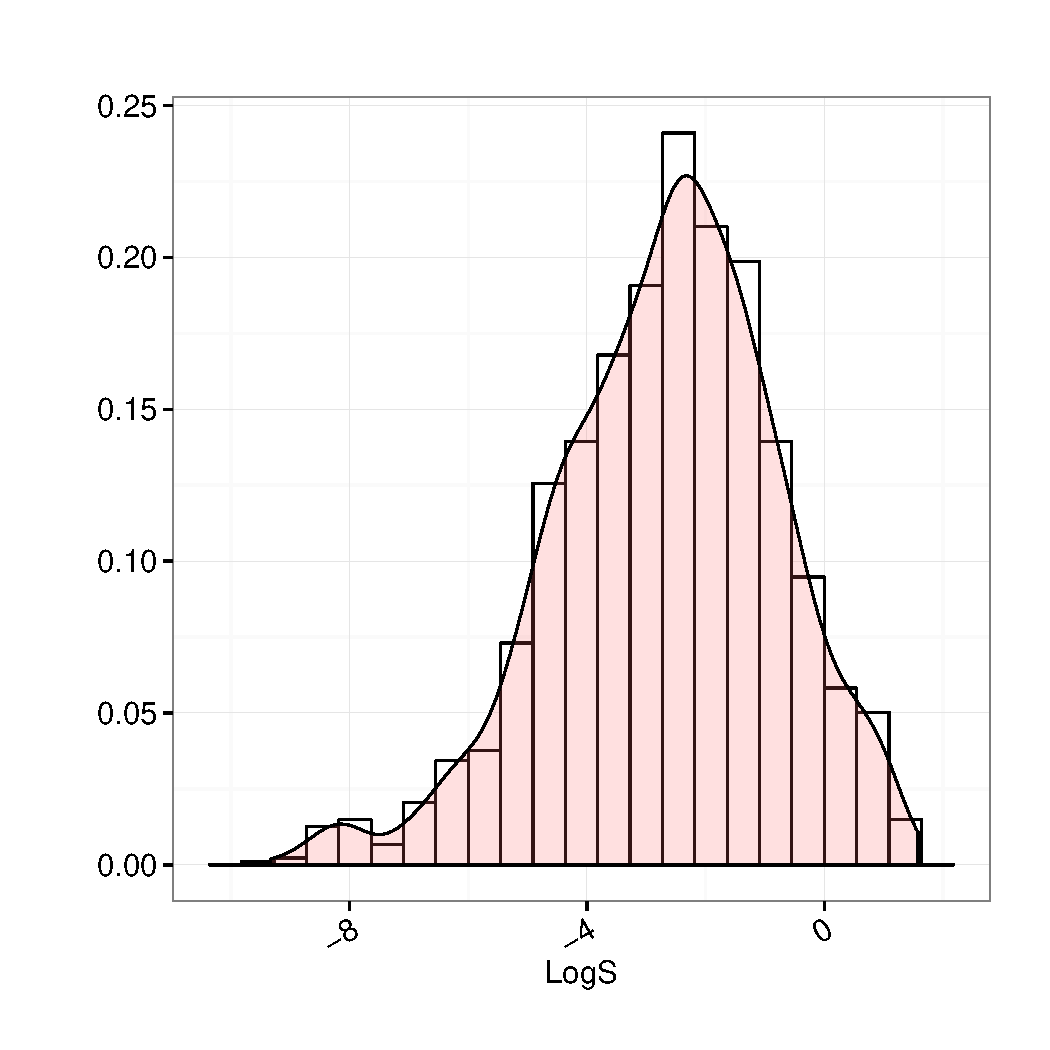
\includegraphics[width=12cm]{figure/unnamed-chunk-6} 

}

\caption[Bioactivity Distribution]{Bioactivity Distribution\label{fig:unnamed-chunk-6}}
\end{figure}


\end{knitrout}


\section{Statistical Pre-processing}
Merge the calculated descriptors and the target values by name into a single data.frame. Check that the number of rows of the merged and original data.frames are the same. Split the data.frame into ids, x and y where ids are the molecule names, x are the descriptor values and y is the target values.  
\begin{knitrout}
\definecolor{shadecolor}{rgb}{0.969, 0.969, 0.969}\color{fgcolor}\begin{kframe}
\begin{alltt}
\hlstd{all} \hlkwb{<-} \hlkwd{merge}\hlstd{(}\hlkwc{x} \hlstd{= targets,} \hlkwc{y} \hlstd{= descriptors,} \hlkwc{by} \hlstd{=} \hlstr{"Name"}\hlstd{)}
\hlcom{# check the number of rows are the same}
\hlkwd{dim}\hlstd{(all)}
\hlkwd{dim}\hlstd{(targets)}
\hlkwd{dim}\hlstd{(descriptors)}
\hlstd{ids} \hlkwb{<-} \hlstd{all}\hlopt{$}\hlstd{Name}
\hlstd{x} \hlkwb{<-} \hlstd{all[}\hlnum{3}\hlopt{:}\hlkwd{ncol}\hlstd{(all)]}
\hlstd{y} \hlkwb{<-} \hlstd{all}\hlopt{$}\hlstd{target}
\end{alltt}
\end{kframe}
\end{knitrout}


Split the dataset into a training (80\%) and a holdout (20\%) set that will be used to assess the predictive ability of the models. Remove the following descriptors: (i) those with a variance close to zero (near-zero variance), and (ii) those highly correlated:
\begin{knitrout}
\definecolor{shadecolor}{rgb}{0.969, 0.969, 0.969}\color{fgcolor}\begin{kframe}
\begin{alltt}
\hlcom{# replace the infinite values with NA and impute}
\hlcom{# the remaining NA values}
\hlstd{x.finite} \hlkwb{<-} \hlkwd{ReplaceInfinitesWithNA}\hlstd{(x)}
\hlstd{x.imputed} \hlkwb{<-} \hlkwd{ImputeFeatures}\hlstd{(x.finite)}

\hlcom{# split the dataset into a training and holdout set}
\hlstd{dataset} \hlkwb{<-} \hlkwd{SplitSet}\hlstd{(ids, x.imputed, y,} \hlkwc{percentage} \hlstd{=} \hlnum{20}\hlstd{)}

\hlcom{# remove the descriptors that are highly correlated}
\hlcom{# or have low variance}
\hlstd{dataset} \hlkwb{<-} \hlkwd{RemoveNearZeroVarianceFeatures}\hlstd{(dataset)}
\hlstd{dataset} \hlkwb{<-} \hlkwd{RemoveHighlyCorrelatedFeatures}\hlstd{(dataset)}
\end{alltt}
\end{kframe}
\end{knitrout}


Center and scale the descriptors:
\begin{knitrout}
\definecolor{shadecolor}{rgb}{0.969, 0.969, 0.969}\color{fgcolor}\begin{kframe}
\begin{alltt}
\hlstd{dataset} \hlkwb{<-} \hlkwd{PreProcess}\hlstd{(dataset)}
\end{alltt}
\end{kframe}
\end{knitrout}


Given that cross-validation (CV) will be used to optimize the hyperparameters of the models, we divide the training setin 5 folds:
\begin{knitrout}
\definecolor{shadecolor}{rgb}{0.969, 0.969, 0.969}\color{fgcolor}\begin{kframe}
\begin{alltt}
\hlstd{dataset} \hlkwb{<-} \hlkwd{GetCVTrainControl}\hlstd{(dataset)}
\hlkwd{saveRDS}\hlstd{(dataset,} \hlkwc{file} \hlstd{=} \hlstr{"dataset.rds"}\hlstd{)}
\end{alltt}
\end{kframe}
\end{knitrout}


\section{Model Training}

\begin{knitrout}
\definecolor{shadecolor}{rgb}{0.969, 0.969, 0.969}\color{fgcolor}\begin{kframe}
\begin{alltt}
\hlcom{# register the number of cores to use in training}
\hlkwd{registerDoMC}\hlstd{(}\hlkwc{cores} \hlstd{=} \hlnum{1}\hlstd{)}

\hlcom{# train and save a support vector machine model}
\hlstd{method} \hlkwb{<-} \hlstr{"svmRadial"}
\hlstd{tune.grid} \hlkwb{<-} \hlkwd{expand.grid}\hlstd{(}\hlkwc{.sigma} \hlstd{=} \hlkwd{expGrid}\hlstd{(}\hlopt{-}\hlnum{8}\hlstd{,} \hlnum{4}\hlstd{,} \hlnum{2}\hlstd{,}
    \hlnum{2}\hlstd{),} \hlkwc{.C} \hlstd{=} \hlkwd{c}\hlstd{(}\hlnum{1e-04}\hlstd{,} \hlnum{0.001}\hlstd{,} \hlnum{0.01}\hlstd{,} \hlnum{0.1}\hlstd{,} \hlnum{1}\hlstd{,} \hlnum{10}\hlstd{,} \hlnum{100}\hlstd{))}
\hlstd{model} \hlkwb{<-} \hlkwd{train}\hlstd{(dataset}\hlopt{$}\hlstd{x.train, dataset}\hlopt{$}\hlstd{y.train, method,}
    \hlkwc{tuneGrid} \hlstd{= tune.grid,} \hlkwc{trControl} \hlstd{= dataset}\hlopt{$}\hlstd{trControl)}
\hlkwd{saveRDS}\hlstd{(model,} \hlkwc{file} \hlstd{=} \hlkwd{paste}\hlstd{(method,} \hlstr{".rds"}\hlstd{,} \hlkwc{sep} \hlstd{=} \hlstr{""}\hlstd{))}

\hlcom{# train and save a random forest model}
\hlstd{method} \hlkwb{<-} \hlstr{"rf"}
\hlstd{tune.grid} \hlkwb{<-} \hlkwd{expand.grid}\hlstd{(}\hlkwc{.mtry} \hlstd{=} \hlkwd{seq}\hlstd{(}\hlnum{5}\hlstd{,} \hlnum{100}\hlstd{,} \hlnum{5}\hlstd{))}
\hlstd{model} \hlkwb{<-} \hlkwd{train}\hlstd{(dataset}\hlopt{$}\hlstd{x.train, dataset}\hlopt{$}\hlstd{y.train, method,}
    \hlkwc{tuneGrid} \hlstd{= tune.grid,} \hlkwc{trControl} \hlstd{= dataset}\hlopt{$}\hlstd{trControl)}
\hlkwd{saveRDS}\hlstd{(model,} \hlkwc{file} \hlstd{=} \hlkwd{paste}\hlstd{(method,} \hlstr{".rds"}\hlstd{,} \hlkwc{sep} \hlstd{=} \hlstr{""}\hlstd{))}

\hlcom{# train and save a gradient boosted machines model}
\hlstd{method} \hlkwb{<-} \hlstr{"gbm"}
\hlstd{tune.grid} \hlkwb{<-} \hlkwd{expand.grid}\hlstd{(}\hlkwc{.n.trees} \hlstd{=} \hlkwd{c}\hlstd{(}\hlnum{500}\hlstd{,} \hlnum{1000}\hlstd{),} \hlkwc{.interaction.depth} \hlstd{=} \hlkwd{c}\hlstd{(}\hlnum{25}\hlstd{),}
    \hlkwc{.shrinkage} \hlstd{=} \hlkwd{c}\hlstd{(}\hlnum{0.04}\hlstd{,} \hlnum{0.08}\hlstd{,} \hlnum{0.16}\hlstd{))}
\hlstd{model} \hlkwb{<-} \hlkwd{train}\hlstd{(dataset}\hlopt{$}\hlstd{x.train, dataset}\hlopt{$}\hlstd{y.train, method,}
    \hlkwc{tuneGrid} \hlstd{= tune.grid,} \hlkwc{trControl} \hlstd{= dataset}\hlopt{$}\hlstd{trControl)}
\hlkwd{saveRDS}\hlstd{(model,} \hlkwc{file} \hlstd{=} \hlkwd{paste}\hlstd{(method,} \hlstr{".rds"}\hlstd{,} \hlkwc{sep} \hlstd{=} \hlstr{""}\hlstd{))}
\end{alltt}
\end{kframe}
\end{knitrout}


\section{Model Evaluation}

Once the models are trained, the cross validated metrics can be calculated:

\begin{knitrout}
\definecolor{shadecolor}{rgb}{0.969, 0.969, 0.969}\color{fgcolor}\begin{kframe}
\begin{alltt}
\hlstd{dataset} \hlkwb{<-} \hlkwd{readRDS}\hlstd{(}\hlstr{"dataset.rds"}\hlstd{)}
\hlstd{model} \hlkwb{<-} \hlkwd{readRDS}\hlstd{(}\hlstr{"svmRadial.rds"}\hlstd{)}

\hlcom{# Cross Validation Metrics.}
\hlkwd{RMSE_CV}\hlstd{(model)}
\end{alltt}
\begin{verbatim}
## [1] 0.632
\end{verbatim}
\begin{alltt}
\hlkwd{Rsquared_CV}\hlstd{(model)}
\end{alltt}
\begin{verbatim}
## [1] 0.8834
\end{verbatim}
\end{kframe}
\end{knitrout}


On the basis of the soundness of the obtained models, we predict the values for the holdout set:
\begin{knitrout}
\definecolor{shadecolor}{rgb}{0.969, 0.969, 0.969}\color{fgcolor}\begin{kframe}
\begin{alltt}
\hlstd{holdout.predictions} \hlkwb{<-} \hlkwd{as.vector}\hlstd{(}\hlkwd{predict}\hlstd{(model,} \hlkwc{newdata} \hlstd{= dataset}\hlopt{$}\hlstd{x.holdout))}
\hlkwd{CorrelationPlot}\hlstd{(}\hlkwc{pred} \hlstd{= holdout.predictions,} \hlkwc{obs} \hlstd{= dataset}\hlopt{$}\hlstd{y.holdout)}
\end{alltt}
\end{kframe}
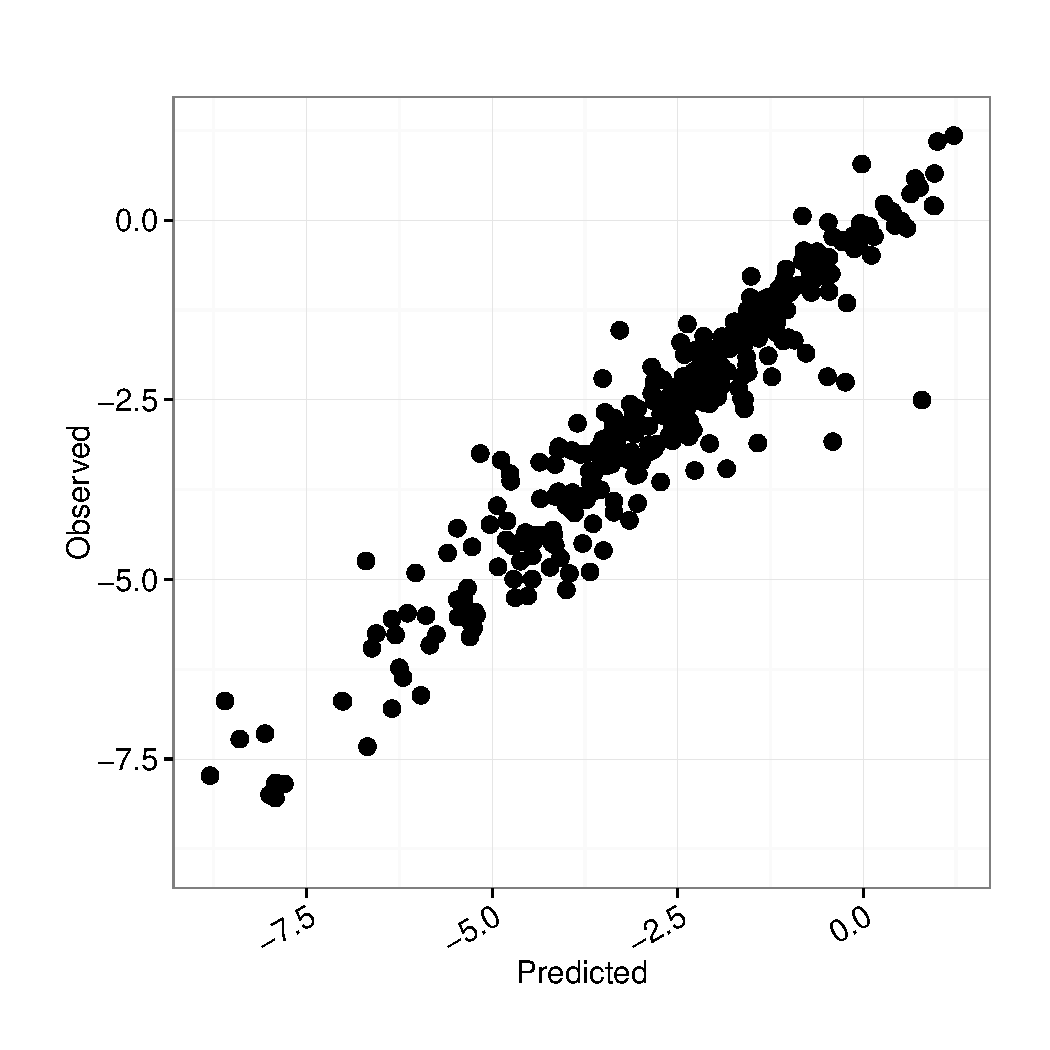
\includegraphics[width=\maxwidth]{figure/unnamed-chunk-13} 

\end{knitrout}


We evaluate the predictive ability of our models by calculation the following statistical metrics:\\

{\bf Internal validation:}
\\
\begin{equation}
q_{{\it int}}^{2} = 1 - \frac {\sum_{i=1}^{N} (y_{i} - \widetilde{y}_{i})^{2}} {\sum_{i=1}^{N} (y_{i} - \bar{y}_{tr})^{2}}
\end{equation}
% cross-validated correlation coefficient

\begin{equation}
RMSE_{int} = \frac {\sqrt {(y_i - \widetilde{y}_i)^{2}}} {N}
\end{equation}

where $N$, $y_i$, $\widetilde{y}_i$ and $\bar{y}_{tr}$ represent the size of the training set, the observed, the predicted and the averaged values of the response variable for those datapoints included in the training set. The {\it i}th position within the training set is defined by {\it i}.  
\\
\\
{\bf External validation:}
\\

\begin{equation}
q_{{\it ext}}^{2} = 1 - \frac {\sum_{j=1}^{N} (y_j-\widetilde{y}_j)^{2}}  {\sum_{j=1}^{N} (y_j - \bar{y}_{ext})^{2}}
\end{equation}

\begin{equation}
RMSE_{ext} = \frac {\sqrt {(y_i - \widetilde{y}_i)^{2}}} {N} 
\end{equation}

\begin{equation}
R_{ext}^{2} = \frac {{\sum_{i=1}^{N} (y_{i} - \bar{y}_{ext})}  (\widetilde{y}_{i} - \overset{-}{\widetilde{y}_{ext}})} 
{\sqrt{\sum_{i=1}^{N} (y_{i} - \bar{y}_{ext})^{2} \sum{ (\widetilde{y}_{i} - \overset{-}{\widetilde{y}_{ext}})^{2}}}}
\end{equation}

\begin{equation}
R_{0\:ext}^2 = 1 - \frac {\sum_{j=1}^{N} (y_{j} - \widetilde{y}_{j}^{ r0})^{2}} {\sum_{j=1}^{N} (y_{j} - \bar{y}_{ext})^{2}} 
\end{equation}

where $N$, $y_j$, $\widetilde{y}_j$, $\bar{y}_{ext}$ and $\breve{y}_j$ represent the size of the training set, the observed, the predicted, the averaged values and the fitted
values of the response variable for those datapoints comprising the external set. The {\it j}th position within the external set is defined by {\it j}. $R_{0\:ext}^2$ is the square of the coefficient of determination through the origin, being $\widetilde{y}_{j}^{ r0} = k \widetilde{y}_j$ the regression through the origin (observed versus predicted) and $k$ its slope.\\
For a detailed discussion of both the evaluation of the predictive ability through the external set and different formulations for $q^{2}$, see ref.\cite{consonni}. 
To be considered as predictive, a model must satisfy the following criteria:\cite{beware,earnest}
\\
\begin{enumerate}
\item $q_{{\it int}}^{2} > 0.5$
\item $R_{ext}^2 > 0.6$
\item $ \frac {(R_{ext}^2 - R_{0\:ext}^2)} {R_{ext}^2} < 0.1$
\item $0.85 \leq k \leq 1.15$
\end{enumerate}

The metrics for the external validatin are given by:
\begin{knitrout}
\definecolor{shadecolor}{rgb}{0.969, 0.969, 0.969}\color{fgcolor}\begin{kframe}
\begin{alltt}
\hlcom{# Statistics for Model Validation}
\hlkwd{Validation}\hlstd{(holdout.predictions, dataset}\hlopt{$}\hlstd{y.holdout)}
\end{alltt}
\begin{verbatim}
## $R2
## [1] 0.9078
## 
## $R02
## [1] 0.907
## 
## $Q2
## [1] 0.907
## 
## $RMSE
## [1] 0.5984
## 
## $Slope
## [1] 1.001
## 
## $MAE
## [1] 0.4101
\end{verbatim}
\end{kframe}
\end{knitrout}


%\section{Bibliography}
%\printbibliography

\end{document}
